\documentclass[10pt, a4paper]{amsart}
% \documentclass[10pt,showpacs,preprintnumbers,footinbib,amsmath,amssymb,aps,prl,twocolumn,groupedaddress,superscriptaddress,showkeys]{revtex4-1}
\usepackage[]{graphicx}
\usepackage[]{hyperref}
\usepackage[]{physics}
\usepackage[]{listings}
\usepackage[T1]{fontenc}
\usepackage{color}
\usepackage[ruled,vlined]{algorithm2e}

\usepackage{amsmath, amsfonts, amssymb}
\usepackage{listings}
\usepackage[]{subcaption}

\newcommand{\erfc}{\text{erfc}}

% Definition of code and how the code should look.
\usepackage{xcolor}
\definecolor{codegreen}{rgb}{0,0.6,0}
\definecolor{codegray}{rgb}{0.5,0.5,0.5}
\definecolor{codepurple}{rgb}{0.58,0,0.82}
\definecolor{backcolour}{rgb}{0.95,0.95,0.92}
\definecolor{mygreen}{rgb}{0,0.6,0}
\definecolor{mymauve}{rgb}{0.58,0,0.82}


\lstdefinestyle{python3}{
    backgroundcolor=\color{backcolour},
    commentstyle=\color{codegreen},
    keywordstyle=\color{magenta},
    numberstyle=\tiny\color{codegray},
    stringstyle=\color{codepurple},
    basicstyle=\ttfamily\footnotesize,
    breakatwhitespace=false,
    breaklines=true,
    captionpos=b,
    keepspaces=true,
    numbers=left,
    numbersep=5pt,
    showspaces=false,
    showstringspaces=false,
    showtabs=false,
    tabsize=2
}
% End def.



\lstset{ %
  backgroundcolor=\color{white},   % choose the background color; you must add \usepackage{color} or \usepackage{xcolor}
  basicstyle=\footnotesize,        % the size of the fonts that are used for the code
  breakatwhitespace=false,         % sets if automatic breaks should only happen at whitespace
  breaklines=true,                 % sets automatic line breaking
  captionpos=b,                    % sets the caption-position to bottom
  commentstyle=\color{mygreen},    % comment style
  deletekeywords={...},            % if you want to delete keywords from the given language
  escapeinside={\%*}{*)},          % if you want to add LaTeX within your code
  extendedchars=true,              % lets you use non-ASCII characters; for 8-bits encodings only, does not work with UTF-8
  frame=single,	                   % adds a frame around the code
  keepspaces=true,                 % keeps spaces in text, useful for keeping indentation of code (possibly needs columns=flexible)
  keywordstyle=\color{blue},       % keyword style
  language=python,                    % the language of the code
  style = python3,
  otherkeywords={*,...},           % if you want to add more keywords to the set
  rulecolor=\color{black},         % if not set, the frame-color may be changed on line-breaks within not-black text (e.g. comments (green here))
  showspaces=false,                % show spaces everywhere adding particular underscores; it overrides 'showstringspaces'
  showstringspaces=false,          % underline spaces within strings only
  showtabs=false,                  % show tabs within strings adding particular underscores
  stepnumber=2,                    % the step between two line-numbers. If it's 1, each line will be numbered
  stringstyle=\color{mymauve},     % string literal style
  tabsize=2,	                     % sets default tabsize to 2 spaces
}

\title[Problem set 1]{Problem set 2: Advection and Diffusion\\
\normalsize{Due: 12 Oct. 2020} \\
  \hrulefill\small{ GEO2300: Fysiske prosesser i geofag }\hrulefill}

\author[Sundberg]{Sigurd Sandvoll Sundberg}
\date{\today}

\begin{document}
\maketitle

\section{Problem 1: Tsunami}
\subsection{a)}
Given a wave with initial disturbance assumed to be Gaussian and propagating to the left, which obeys the following equation in 1D:
\begin{equation}\label{eq:pr1}
	\frac{\partial }{\partial t} h - c_0 \frac{\partial}{\partial x}h = 0
\end{equation}
We want to write the expression of the moving wave, when the following is given 
\begin{itemize}
	\item $c_0 = 700 km/hr$
	\item $x_0 = 0$
	\item $ A = 1.0m$
	\item Standard deviation $= 50km$
\end{itemize}
Which gives us that at $t = 0$:
\begin{equation}\label{eq:h}
	h = 1.0 \exp(-\frac{x^2}{50^2})
\end{equation}

The solution to equation \ref{eq:pr1} is given by 
\begin{equation}
	h = F(x+c_0t)
\end{equation}
in our case. Given the initial condition \ref{eq:h} when $t = 0$, being initially a Gaussian function, on the form  
\begin{equation}
	\phi(x,0) = \phi_0\exp\left[-(x-x_0)^2/L^2\right]
\end{equation}
then our solution becomes 
\begin{equation}
	h(x,t) = 1.0 \exp\left(-\frac{(x+c_0t)^2}{50^2}\right)
\end{equation}
\subsection{b)}
We want to find the finite difference form, using the FTCS scheme for equation \ref{eq:pr1}. 
This is given by Taylor expansion around the first degree term, and reads as follows 
\begin{align}\label{1FTCS}
	\frac{h_j^{n+1} - h_j^n}{\Delta t} &- c_0 \frac{h_{j+1}^n - h_{j-1}^n}{2\Delta x} = 0 && \text{Rearrange for $h_j^{n+1}$}\\
	h_j^{n+1} &= \frac{C}{2}h_{j+1}^n + h_j^n - \frac{C}{2}h_{j-1}^n && \text{Where $C = \frac{c_0\Delta t}{2\Delta x}$}
\end{align}
We have here defined $h_j^n$ as the following:
\begin{itemize}
	\item $h(t,x) \simeq h(t_n, x_j) = h_j^n$ 
	\item $t_n$ is the time partitioned into $n$ equally sized time steps. 
	\item $x_j$ is the distance partitioned into $j$ equal steps. 
	\item $\Delta t = t_{n+1} - t_n$ 
	\item $\Delta x = x_{j+1} - x_j$
\end{itemize} 
\subsection{c)}
Given the following Neumann boundary conditions 
\begin{equation}
	\frac{\partial }{\partial x}h = 0
\end{equation}
This gives that 
\begin{align}
	h_{-1} &= h_0 \\
	h_{n+1} &= h_{n}
\end{align}
for $n$ grid points. Where we have ghost points that follows the above equations. 

Let $n = 6$, i.e. $j = 0,1,2,3,4,5,6$, be the number of grid points. Our set of equations then become 
\begin{align}
	h_0^{n+1} &= \frac{C}{2}h_1^n + h_0^n - \frac{C}{2}h_0^n && \text{Here $h_0 = h_{-1}$}\\
	h_1^{n+1} &= \frac{C}{2}h_2^n + h_1^n - \frac{C}{2}h_0^n\\
	h_2^{n+1} &= \frac{C}{2}h_3^n + h_2^n - \frac{C}{2}h_1^n\\
	h_3^{n+1} &= \frac{C}{2}h_4^n + h_3^n - \frac{C}{2}h_2^n\\
	h_4^{n+1} &= \frac{C}{2}h_5^n + h_4^n - \frac{C}{2}h_3^n\\
	h_5^{n+1} &= \frac{C}{2}h_6^n + h_5^n - \frac{C}{2}h_4^n\\
	h_6^{n+1} &= \frac{C}{2}h_6^n + h_6^n - \frac{C}{2}h_5^n && \text{Here $h_6 = h_7$}
\end{align}
This gives us a tridiagonal matrix on the following form, for a given $n$. 
\begin{equation}
	\begin{bmatrix}
		1-\frac{C}{2} & \frac{C}{2} & 0 & 0 & 0 & 0 & 0\\
		- \frac{C}{2} & 1 & \frac{C}{2} & 0 & 0 & 0 & 0\\
		0 & - \frac{C}{2} & 1 & \frac{C}{2} & 0 & 0 & 0\\
		0 & 0 & - \frac{C}{2} & 1 & \frac{C}{2} & 0 & 0\\
		0 & 0 & 0 & - \frac{C}{2} & 1 & \frac{C}{2} & 0\\
		0 & 0 & 0 & 0 & - \frac{C}{2} & 1 & \frac{C}{2}\\
		0 & 0 & 0 & 0 & 0 & - \frac{C}{2} & 1 + \frac{C}{2}
	\end{bmatrix}
\end{equation}
This can easily be extended to a arbitrary $n \times n$ matrix. 

\subsection{d)}
The code in \ref{pr1d} implements the FTCS scheme found above for the following conditions 
\begin{itemize}
	\item $x \in [-1400, 300]$, with unit km.
	\item $n = 400$ grid points.
	\item $c_0 = 700$ kmh.
	\item $C = c_0 dt/dx = 0.1$
	\item $dt = Cdx/c_0$
\end{itemize}
\lstinputlisting[label=pr1d]{"../code/pr1_d.py"}

\subsection{e)}
Seen in figure \ref{fig:1e} we see the numerical solutions plotted against the analytical solutions for time values $t = 0,0.5,1,1.5,2$. We see that the FTCS scheme is unstable when plotting the wave equation, as seen in the out bursts seen above and below the black curve. However is still reproduces the results to a fairly okay, and gives an easy way to get an idea of the solutions to the problem. Before choosing a more appropriate scheme for the problem at hand. 
\begin{figure}[h]
\centering
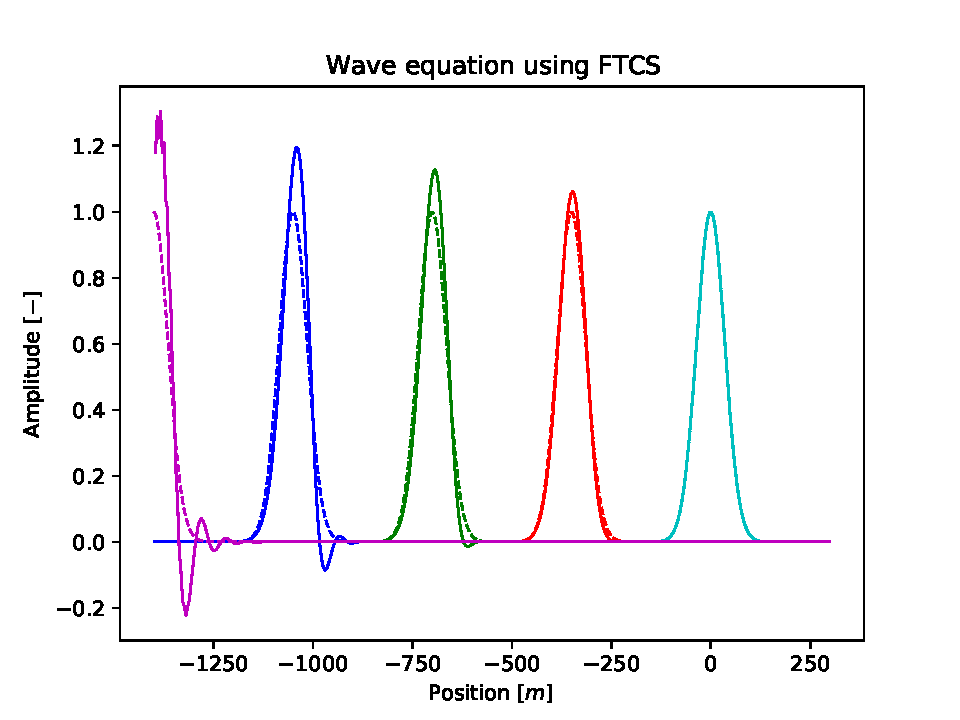
\includegraphics[width=0.9\linewidth]{"../code/FTCS.pdf"}
\caption{Plot of the analytical solution to the wave equation against the FTCS scheme for the numerical solution. The time values are shown from left to right, so the far most left top is for t = 0, and the right most top is for t = 2. Numerical is shown in full line, and the analytical is shown as dashed line.}
\label{fig:1e}
\end{figure}

\subsection{f)}
The Crank-Nicholson(CN) scheme is a combination of the FTCS scheme shown in \ref{1FTCS} and the iFTCS scheme shown \ref{1iFTCS}.
\begin{equation}\label{1iFTCS}
	-\frac{C}{2}h_{j+1}^{n+1} + h_j^{n+1} +\frac{C}{2}h_{j-1}^{n+1} = h_j^n
\end{equation}
Combining FTCS and iFTCS schemes, in equal parts the CN scheme reads as follows 
\begin{equation}
	- 	\frac{C}{4}h_{j+1}^{n+1} + h_j^{n+1} + 	\frac{C}{4}h_{j-1}^{n+1} = 	\frac{C}{4}h_{j+1}^n + h_j^n - 	\frac{C}{4}h_{j-1}^n
\end{equation}
Writing this on the same form as we did for FTCS scheme we get two matrices for solving the following equation
\begin{equation}\label{eq:CN}
	Bh^{n+1} = Ah^n
\end{equation}
where $A$ and $B$ are our two matrices. Matrix $A$ reads as for FTCS scheme, with all the elements $	\frac{C}{2} \rightarrow 	\frac{C}{4}$. Then matrix $B$ read as follows 
 \begin{equation}
 	\begin{bmatrix}
 		1 + \frac{C}{4} & -\frac{C}{4} & 0 & 0 & 0 & 0 & 0\\
 		 \frac{C}{4} & 1 & -\frac{C}{4} & 0 & 0 & 0 & 0\\
 		0 &  \frac{C}{4} & 1 & -\frac{C}{4} & 0 & 0 & 0\\
 		0 & 0 &  \frac{C}{4} & 1 & -\frac{C}{4} & 0 & 0\\
 		0 & 0 & 0 &  \frac{C}{4} & 1 & -\frac{C}{4} & 0\\
 		0 & 0 & 0 & 0 &  \frac{C}{4} & 1 & -\frac{C}{4}\\
 		0 & 0 & 0 & 0 & 0 &  \frac{C}{4} & 1 - \frac{C}{4}
 	\end{bmatrix}
 \end{equation}
This gives us the ability to solve \ref{eq:CN} the following way 
\begin{equation}
	h^{n+1} = B^{-1}Ah^n
\end{equation}
where $B^{-1}$ is the inverse matrix of $B$. 

\subsection{g)}
Using the same conditions as for problem e). We see from figure \ref{fig:1g} that we have a better numerical solution compared to the FTCS scheme. Our solution is fairly steady above the analytical solution, without increasing as it did for FTCS. However we still see artifacts of the numerical solution, as seem especially for the last time, $t = 2$. This is from the scheme not being that well suited to deal with wave equation when number of iterations grows large. 
\lstinputlisting[label=pr1d]{"../code/pr1_g.py"}
\begin{figure}[h]
	\centering
	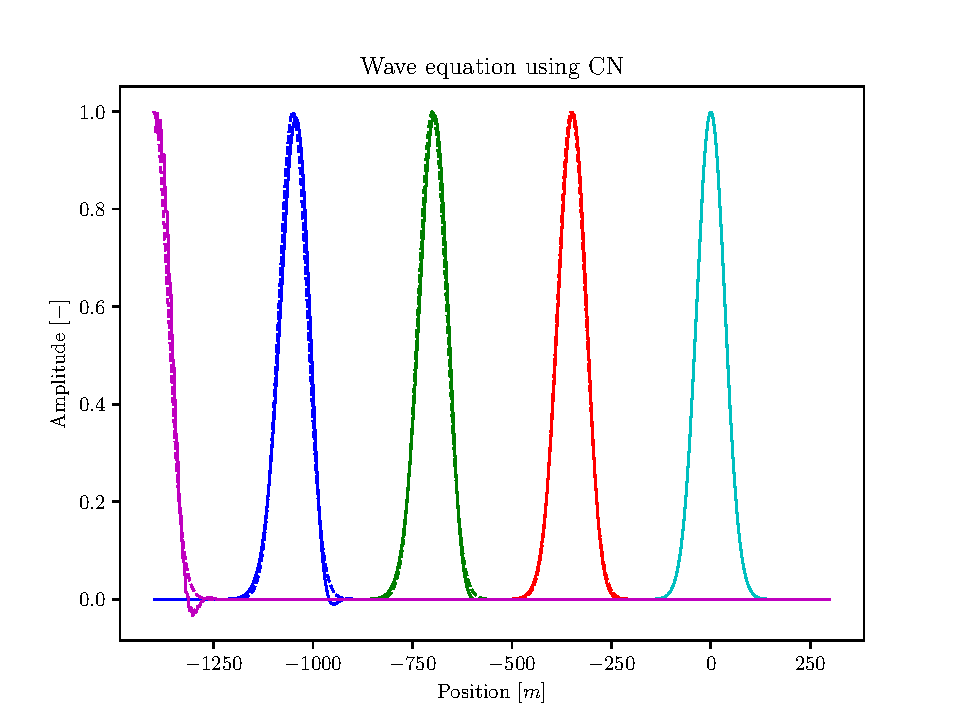
\includegraphics[width=0.9\linewidth]{"../code/CN.pdf"}
	\caption{Plot of the analytical solution to the wave equation against the CN scheme for the numerical solution. The time values are shown from left to right, so the far most left top is for t = 0, and the right most top is for t = 2. Numerical is shown in full line, and the analytical is shown as dashed line.}
	\label{fig:1g}
\end{figure}

\section{Problem 2: Boundary Diffusion}
We will now be looking at a one dimensional aquifer with oil seeping into one end. The oil concentration obeys the 1D diffusion equation
\begin{equation}
	\frac{\partial }{\partial t}C = D \frac{\partial^2}{\partial x^2} C
\end{equation}
\subsection{a)}
We want to find the analytical solution for $C(x,t)$ assuming, $C = C_0$ at $x = 0$ and that $C(x,0) = 0$. 

The analytical solution follows as from the compendium\cite{comp} is 
\begin{equation}
	C = C_0\erfc\left(\frac{x}{2\sqrt{Dt}}\right)
\end{equation}
\subsection{b)}
The following program is used to find the answers in both problem b) and c). It finds the oil concentration at times $t = 1, 10, 100$ days, with $C_0 = 0.5$. 
\lstinputlisting[label=pr2b]{"../code/pr2_b_c.py"}

The concentration as a function of time is seen in figure \ref{fig:2b}, where we see what is expected with a large part of the aquifer being filled with oil after a longer period of time. 
\begin{figure}[]
	\centering
	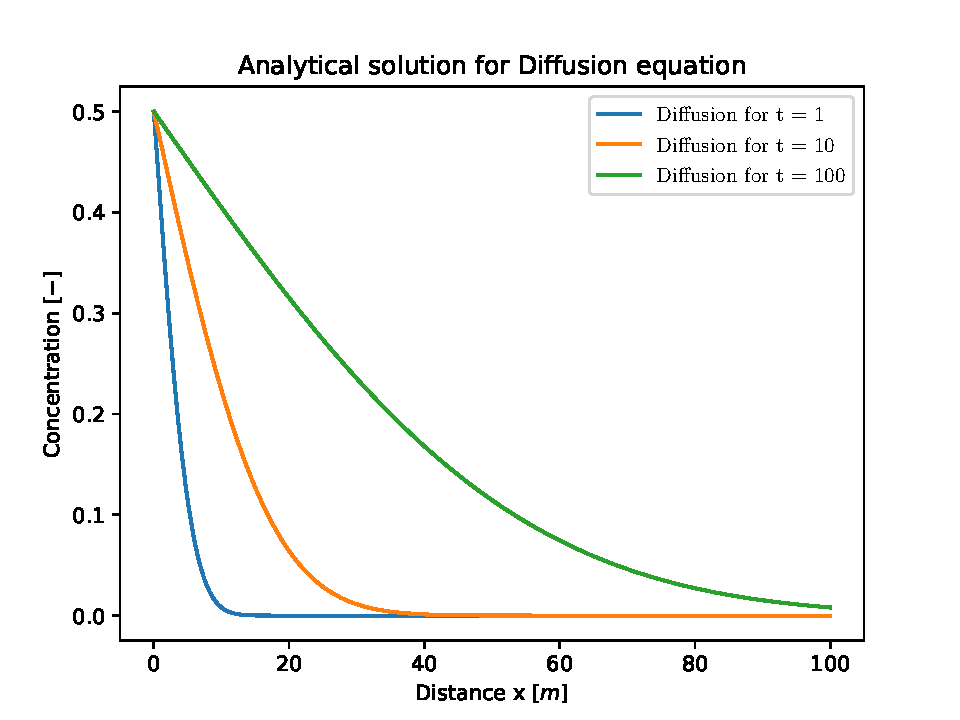
\includegraphics[width=0.9\linewidth]{"../code/FTCS2.pdf"}
	\caption{Plot of the analytical solution to the 1D diffusion equation for a aquifer which is 100m long..}
	\label{fig:2b}
\end{figure}
\subsection{c)}
Using the same code as in b), we want to find when the concentration reaches $25\%$ at distance $x = 100$m and $x = 1000$m from the source. Also how much longer do you have to wait if the distance is increased by a factor of $\alpha$. 

Running our program we get the following output
\begin{lstlisting}
	"""
	Number of days needed for the concentration to reach 25% is: 1273 days, with x = 100
	Number of days needed for the concentration to reach 25% is: 127206 days, with x = 1000
	"""
\end{lstlisting}
The relation between these two is roughly a factor of 100, with an increase in distance of a factor of 10. However this does not tell us really tell us the relation, however running more iterations for different values of $x$, we find the results which can be seen in \ref{fig:rel}
\begin{figure}[]
	\centering
	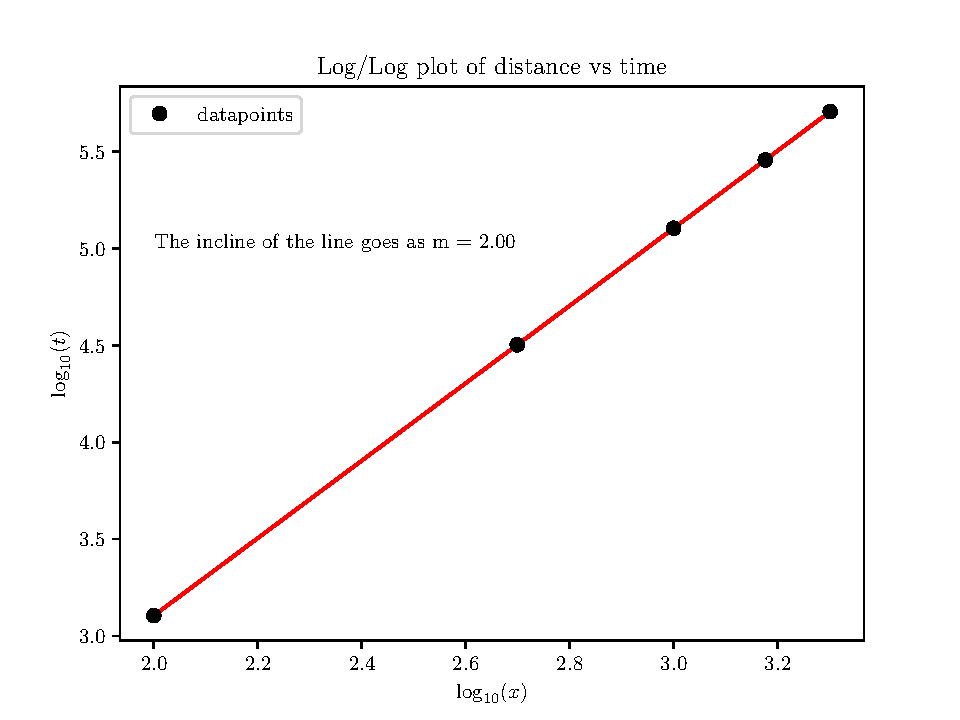
\includegraphics[width=0.9\linewidth]{"../code/Relation.pdf"}
	\caption{Plot for different values of $x$ against the respective number of days.}
	\label{fig:rel}
\end{figure}
From here we can see that the relation follows a logarithmic scale, of $\log_{10}$. Such that our relation goes as 
\begin{equation}
	\log_{10}(x) = 2\log_{10}(t)
\end{equation}
or 
\begin{equation}
	x = t^2
\end{equation}
So for any a given $\alpha_x$ we have the following relation $\alpha_x \propto \alpha_t^2$. Where $\alpha_x$ and $\alpha_t$ is the increase in position and time, respectively by a factor $\alpha$
\subsection{d)}
Writing up the FTCS scheme we have the following base expansion 
\begin{align}
	\frac{C^{n+1}_j - C_j^n}{dt} &= D \frac{C_{j+1}^n-2C_j^n+C_{j+1^n}}{dx^2}\\
	C_j^{n+1} &= sC_j{+1}^n + (1-2s)C_j^n + sC_{j-1}^n && \text{With $s = \frac{D \, dt}{dx^2}$}
\end{align}
Expanding this with 7 grid points, and using $C(x=0) = 0.5 \land C(x=100) = 0$ we have 
\begin{align}
	C_0^{n+1} &= 0.5 \\
	C_1^{n+1} &= sC_0^n + (1-2s)C_1^n + sC_2^n\\
	C_2^{n+1} &= sC_1^n + (1-2s)C_2^n + sC_3^n\\
	C_3^{n+1} &= sC_2^n + (1-2s)C_3^n + sC_4^n\\
	C_4^{n+1} &= sC_3^n + (1-2s)C_4^n + sC_5^n\\
	C_5^{n+1} &= sC_4^n + (1-2s)C_5^n + sC_6^n\\
	C_6^{n+1} &= 0
\end{align}
From this we can construct a matrix $A$ such that we can solve the following equation 
\begin{equation}
	C^{n+1} = A C^n
\end{equation}
\subsection{e)}
The following code implements the FTCS scheme with N grid points. 
\lstinputlisting[label=pr2b]{"../code/pr2_e.py"}
We can see from figure \ref{fig:diff} that for t = 1 that our solution agrees extremely well with the analytical solution, is there is no visible difference between the two graphs. For higher values of t, namely t = 10 and t = 100, we see that our numerical solution strays further from the analytical one. What is notable is that for t = 100, our numerical solution reproduces the exponential function poorly as our difference scheme is based around a second order polynomial. Importantly this means that for higher values of t>100, we would no longer get solutions which represents the analytical one. This means that for low values of t, we can reproduce the analytical results, but for higher values of t, we would need a more appropriate scheme, to predict the analytical results. 
\begin{figure}[h]
	\centering
	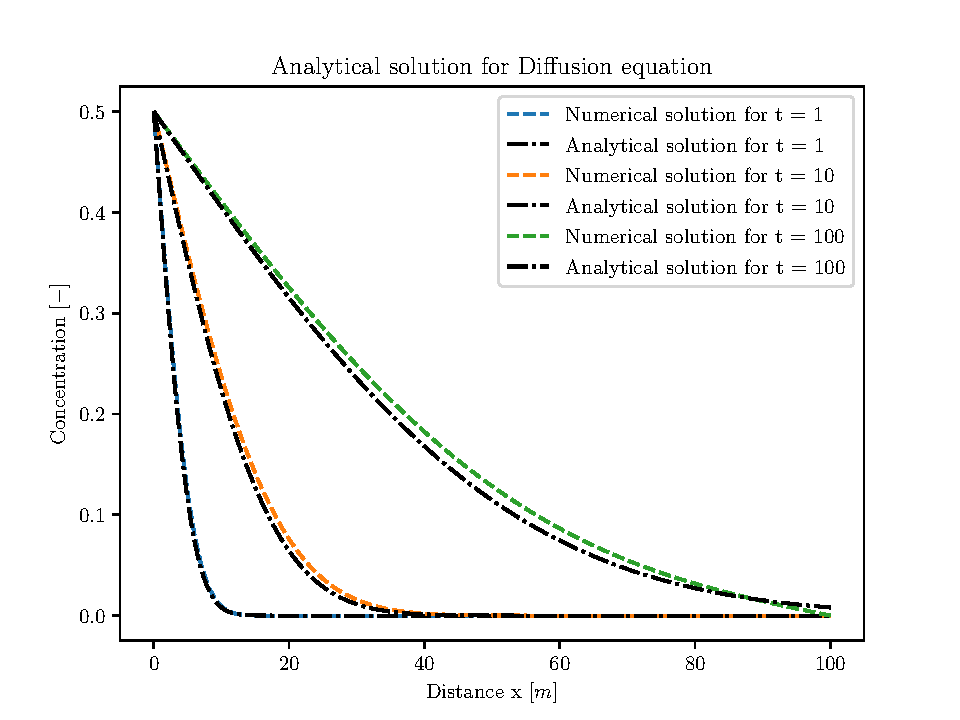
\includegraphics[width=0.9\linewidth]{"../code/NUMFTCS.pdf"}
	\caption{Plot of the analytical solution and numerical solution to the 1D diffusion equation, with s = 0.4.}
	\label{fig:diff}
\end{figure}
\subsection{f)}
We see that when we choose s = 0.6 that our solution blows up as is expected from the stability of the FTCS scheme. We can also see that for higher values of t that the solution blows up more. This is because how much a solution blows up is dependent on the number of iterations which is performed on the data set. All solutions blow up, but we can only see the effects of the higher time step when plotting them in the same plot. This results can be seen in \ref{fig:ex}. 
\begin{figure}[h]
	\centering
	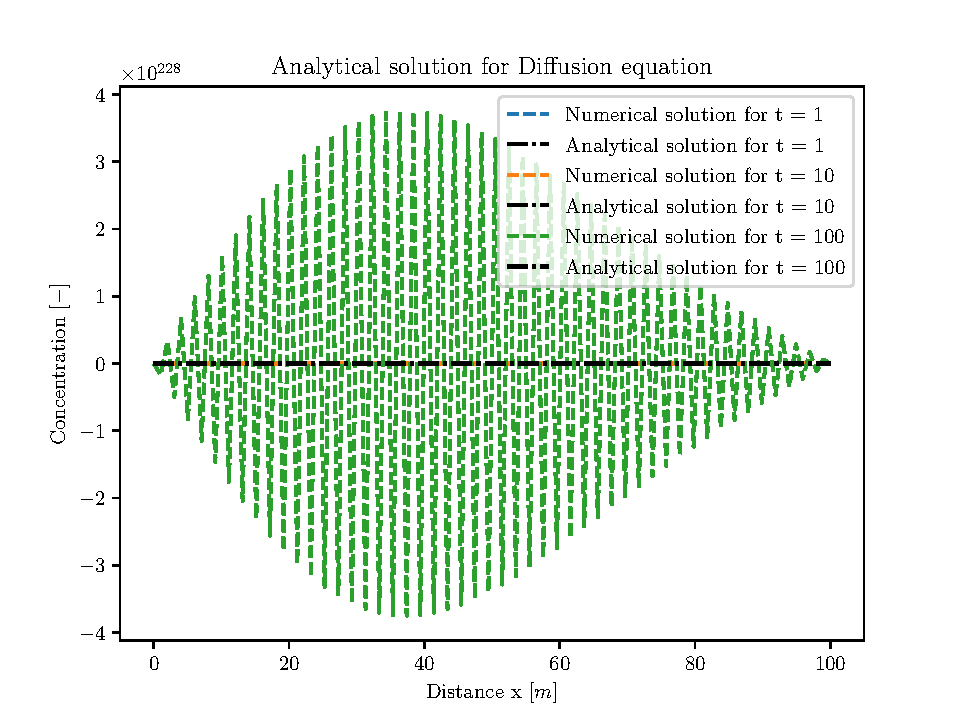
\includegraphics[width=0.9\linewidth]{"../code/exNUMFTCS.pdf"}
	\caption{Plot of the analytical solution and numerical solution to the 1D diffusion equation, with s = 0.6.}
	\label{fig:ex}
\end{figure}

\begin{thebibliography}{1}
	\bibitem{comp} 
	Joe LaCasce. 
	\textit{Physical Processes in the Geosciences}. 
	Department of Geosciences, University of Oslo, Norway. 
	Downloaded: 25.09.2020
\end{thebibliography}
%\lstinputlisting[label=tridiag]{"../code/tridiag.py"}


\end{document}
